\documentclass{article}
\usepackage[colorlinks=true, citecolor=teal, linkcolor=Periwinkle, urlcolor=Periwinkle]{hyperref}
\usepackage[dvipsnames]{xcolor}
\usepackage{graphicx}

\linespread{1.15}
\bibliographystyle{ieeetr}

\title{Perceptual Losses for Real-Time Style~Transfer and~Super-Resolution}
\author{Iantsa~Provost, Lilian~Rebiere, Bastien~Soucasse, and~Alexey~Zhukov}
\date{January~5, 2022}

\begin{document}

% Title page
{
    \begin{titlepage}
        \begin{center}
            \vspace*{1.5cm}
            
            \Large
            
            \textbf{Perceptual Losses for Real-Time Style~Transfer and~Super-Resolution}
            
            \vspace{.5cm}
            
            \vspace{1.5cm}
            
            \large
            
            \textbf{Iantsa~Provost, Lilian~Rebiere, Bastien~Soucasse, and~Alexey~Zhukov}
            
            \vfill
            
            \normalsize
            
            Presented as part of the\\
            \textit{AMIP}\\
            course unit.
            
            \vspace{1.5cm}
            
            
\includegraphics[width=.5\textwidth]{images/college-logo.jpg}
            
            Computer~Science~Master's~Degree in~Image~and~Sound\\
            Université~de~Bordeaux,~France\\
            January~5,~2022
        \end{center}
    \end{titlepage}
    \newpage
    \setcounter{page}{2}
}

% Table of Contents
{
    \hypersetup{linkcolor=black}
    \tableofcontents
    \newpage
}

% Introduction
{
    \section{Introduction}
    \label{sec:introduction}

    Johnson~et~al.~\cite{https://doi.org/10.48550/arxiv.1603.08155} introduced a model…

    % Super-resolution techniques are used to reconstruct high-resolution images from low-resolution versions. These methods have a wide range of applications, including image processing, computer vision, and medical imaging. In this report, we describe the implementation and evaluation of a super resolution model that utilizes perceptual losses. This approach was introduced in the paper "Perceptual Losses for Real-Time Style Transfer and Super-Resolution" by J. Johnson et al. Perceptual losses are designed to capture the high-level features of images and maintain the perceptual quality of the recovered images.

    % To train the model, we used a dataset of high-resolution images. We implemented the model and used this dataset for training.

    % In this report, we present and explain the method used in the model, describe any implementation difficulties that we encountered, and analyze the qualitative and quantitative results of the experiments. We also discuss the energy consumption used during the project and consider other possible impacts. Finally, we suggest possible extensions and future directions for this work.


}

% Method Implementation
{
    \section{Method Implementation}
    \label{sec:method-implementation}

    …
}

% Experiments
{
    \section{Experiments}
    \label{sec:experiments}

        \subsection{Set up}

        In order to conduct experiments, we first need a dataset to train our model. The original paper~\cite{https://doi.org/10.48550/arxiv.1603.08155} used the MS COCO dataset \cite{mscoco} for training, but due to its large size and the associated training time, we had to find a more adequate dataset.
        
        As an alternative, we chose DIV2K, a dataset introduced in 2017 by Agustsson et al. in the technical report \textit{"NTIRE 2017 Challenge on Single Image Super-Resolution: Dataset and Study"} ~\cite{div2k-ds}. DIV2K is a widely-used dataset for super resolution tasks containing 1000 pairs of low resolution (LR) and high resolution (HR) images. Compared to the MS COCO dataset, it has a reasonable size, making it more feasible for use in this study. More specifically, we only used the HR Images Train Data, which contains 800 images of variable sizes. An extract is visualizable in Fig.~\ref{fig:div2k-train}.

        \bigskip

        As the model needs a specific type of training data, we did not use the LR images of DIV2K. Indeed, we decided to process the HR images to create our HR-LR pairs. %Furthermore, it allows to store fewer images?

        To do so, the HR images were preprocessed according to the methods described in ~\cite{https://doi.org/10.48550/arxiv.1603.08155}. It includes cropping to $288 \times 288$, blurring with a Gaussian kernel of width $\sigma = 1.0$, and downsampling with bicubic interpolation.
        
        Now that the dataset has been preprocessed, the model and prepared dataset are now ready to be used for training.

        \begin{figure*}[ht]
            \centering
            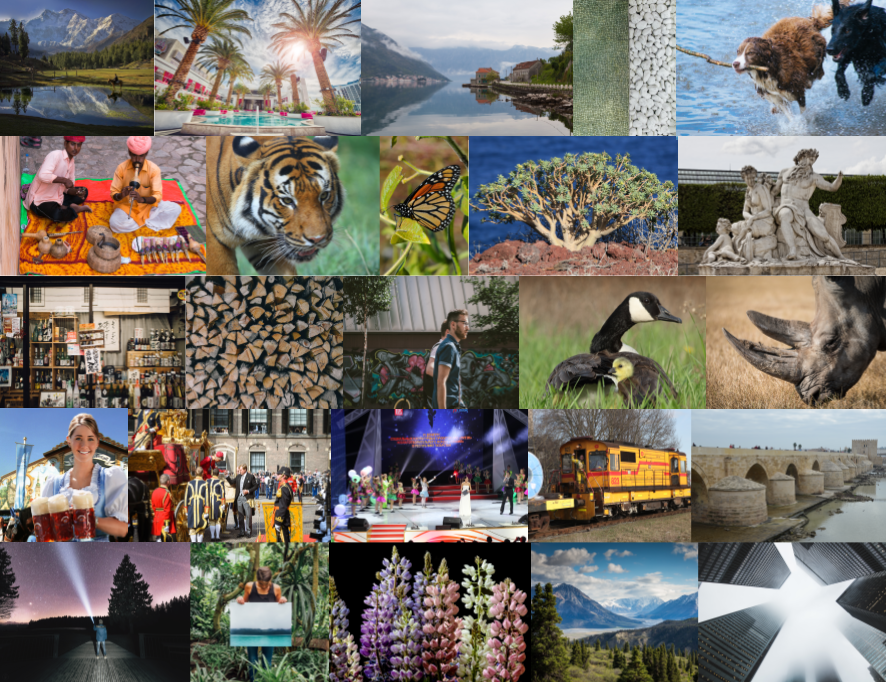
\includegraphics[width=\textwidth]{images/DIV2K_HR.png}
            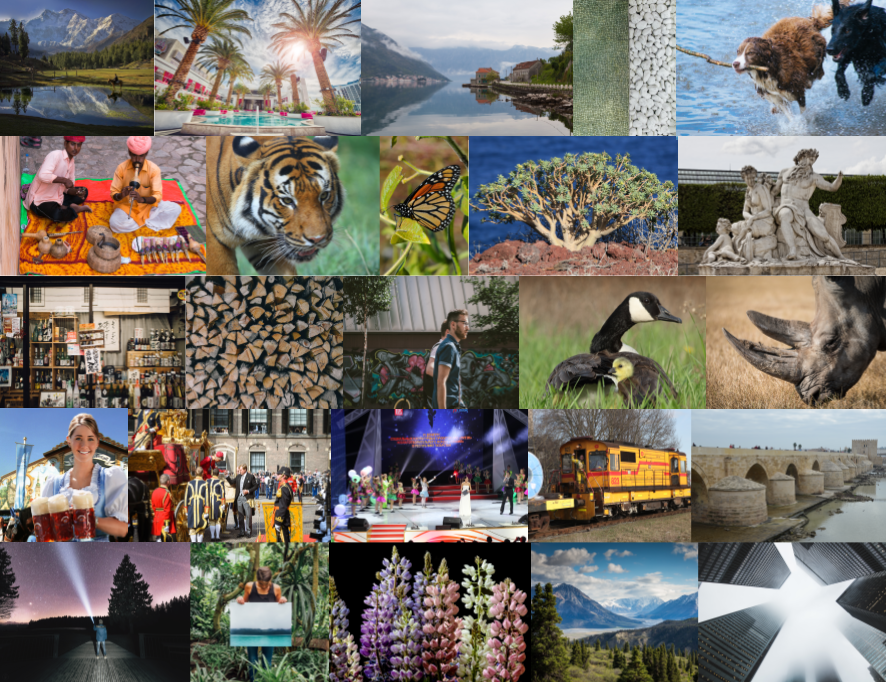
\includegraphics[width=\textwidth]{images/DIV2K_HR.png}
            \caption{Visualization of 25 DIV2K HR train images, and their LR version processed by us.}
            \label{fig:div2k-train}
        \end{figure*}
        % TODO: create such extracts

        % In order to conduct experiments on the super resolution part of the model introduced in the paper "Perceptual Losses for Real-Time Style Transfer and Super-Resolution" by J. Johnson et al., the model was implemented and the DIV2K dataset was prepared for use in training. The original paper used the MS COCO dataset for training, but due to its large size and the associated training time, the DIV2K dataset was selected as an alternative. The DIV2K dataset was chosen because it is a widely-used dataset for super resolution tasks and has a reasonable size, making it more feasible for use in this study. The DIV2K dataset was preprocessed according to the methods described in the paper, including cropping to 288x288, blurring with a Gaussian kernel of width 1, and downsampling with bicubic interpolation. The resulting preprocessed dataset was then loaded into the PyTorch program using the appropriate dataset and dataloader classes. With the model and prepared dataset in place, experiments on the super resolution part of the model can now be carried out.
        
    …
}

% Environmental Impact
{
    \section{Environmental Impact}
    \label{sec:env-impact}

    …
}

% Conclusion
{
    \section{Conclusion}
    \label{sec:conclusion}

    …
}

% References
{
    \bibliography{refs}
}

\end{document}
